\setcounter{ExampleCounter}{1}
What if I told you the average age for a group of 5 people was 
25? Without giving you any more information, you would not be able to guess the five individual ages. One possible set of ages could be 10, 10, 25, 40, 40. Another possible set of ages could be 25, 25, 25, 25, 25. Yet another possible set of ages could be 5, 5, 5, 10, 100.  The mean for each of these data sets is 25, yet the individual values are very different. This is where the spread of the data becomes very important. If we know how much spread there is in the data, we can have a much better idea of what the data set really looks like. In this section, you will learn the different measures of spread. 

\subsection{The Range}
The \textbf{range} is the simplest measure of spread. It is simply the highest data value minus the lowest data value, or the maximum minus the minimum. 

\begin{formula}{Range}
The range is $Maximum - Minimum$
\end{formula}

\begin{example}[https://www.youtube.com/watch?v=mIqrQ6aBJ6I]{Ages}
Let's examine our group of five people again. Below are their possible ages. Calculate the range for each of the data sets below.
\begin{enumerate}[a.]
\item{10, 10, 25, 40, 40}
\item{25, 25, 25, 25, 25}
\item{5, 5, 5, 10, 100}
\end{enumerate}

\marginnote{\bfseries Solution}
\begin{enumerate}[a.]
\item{$Range = Max - Min = 40 - 10 = 30$}
\item{$Range = Max - Min = 25 - 25 =  0$}
\item{$Range = Max - Min = 100 - 5 = 95$}
\end{enumerate}
\end{example}

As you can see from the example above, even though each data set has a mean of 25, the ranges are wildly different. The higher the range, the more spread out the data. The first data set has some spread, the second data set has no spread (hence a range of 0), and the third data set has a lot of spread.

\begin{try}[http://www.izzomath.com/103text/stats/example3.1/story.html]
The number of books checked out from the library from 25 students are as follows:\begin{center}
\begin{tabular}{c c c c c c c c c c}
0 & 0 & 0 & 1 & 2 & 3 & 3 & 4 & 4 & 5\\
5 & 7 & 7 & 7 & 7 & 8 & 8 & 8 & 8 & 9\\
10 & 10 & 11 & 11 & 12 & & & & &
\end{tabular}
\end{center}
Find the range.
\end{try}

Unfortunately, the TI Calculator will not calculate the range for you. However, the 1-VAR-STATS option will give you the maximum and minimum data values, from which you can easily get the range.
\pagebreak

\subsection{The Five Number Summary}
Another way to observe how a data set is spread out is to calculate the \textbf{quartiles}.  The quartiles are similar to the median: the 1st quartile is the data value that is a quarter of the way through the set; the 2nd quartile is the median, halfway through the set; and the 3rd quartile is three quarters of the way through the set.  If you look at the 1-VAR-STATS on the TI calculator, you'll notice $Q_1$ (the 1st quartile) and $Q_3$ (the 3rd quartile) listed.

If you put the three quartiles together with the minimum and maximum of the data set, these form what is known as the \textbf{five number summary}.  They split the data into quarters (Min $\to$ $Q_1$, $Q_1 \to Q_2$, etc.) where each quarter contains a fourth of the data points.  This can provide a good picture of whether the data is clustered on the lower end or on the higher end, or whether it is symmetric or clustered in the middle.

\begin{proc}{Boxplots}
We can display the five number summary visually with a \textbf{boxplot}.  A boxplot consists of a box drawn from the first to the third quartile, with a line at the median, or second quartile.  Lines, or whiskers, extend from this box down to the minimum and up to the maximum (we can also use the quartiles to find outliers and mark them on a boxplot, but we'll omit that here).

The TI calculator can do this for you, if you choose the boxplot option when setting up the STAT PLOT.
\begin{center}
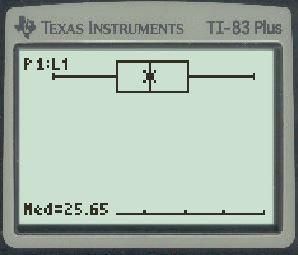
\includegraphics{Calc6}
\end{center}
By using the TRACE function, you can see the minimum, maximum, and quartiles.
\end{proc}

\subsection{The Standard Deviation}

The \textbf{standard deviation} is a number that measures how far a typical data value is from the mean. The standard deviation is always positive or zero. A small standard deviation means less spread in the data; a large standard deviation means more spread in the data.\\

First of all, the \textbf{deviation} of each data point $x$ is its difference from the mean $\overline{x}$:
\[x-\overline{x}.\]
Each value in the data set has a deviation associated with it.  If we want to find how far, on average, each data point is from the mean, it would make sense to take the average of the deviations.  However, there's a problem with doing that: if we add up the deviations, we'll always get 0, because of the way that $\overline{x}$ is calculated.  Some of the deviations are positive, some are negative, and the positives cancel out the negatives.

To get around this, we square the deviations so that everything becomes positive.  NOW, when we take an average\footnote{\textit{almost}} of these \textit{squared} deviations, we get a meaningful number, instead of getting 0 every time.  We call this ``average'' the variance:\marginnote{It is not quite an average, since we divide by $n-1$ instead of $n$.  The reasons for this are complicated, but they have to do with making the sample variance be what is called an unbiased estimator for the population variance.  You can ignore this note except to remember to divide by $n-1$.}
\[s^2 = \dfrac{\sum (x-\overline{x})^2}{n-1}\]

The only problem now is that we've got an average of these squared things, so the units of our answer are not the same units we started with.  In other words, if the data is given in units of inches, we've got a variance in square inches.  To get an answer, we take the square root of the variance, and that's what we call the standard deviation.
\[\textrm{s} = \sqrt{\frac{\Sigma (x - \overline{x})^2}{n-1}}\]

To calculate the standard deviation,
\begin{enumerate}
\item Calculate the mean of the data values, $\overline{x}$.
\item Subtract the mean from each data value to find the deviations: 
\[\textrm{deviation } = x - \overline{x}\]
\item Square each deviation: $(x - \overline{x})^2$
\item Take the sum of the squared deviations: $\Sigma (x - \overline{x})^2$
\item Divide that sum by $n$ minus 1, where $n$ is the number of data values: $\frac{\Sigma (x - \overline{x})^2}{n-1}$
\item Take the square root of this quotient: $\sqrt{\frac{\Sigma (x - \overline{x})^2}{n-1}}$
\end{enumerate}

\begin{formula}{Standard Deviation}
The standard deviation of a sample is given by
\[\textrm{s} = \sqrt{\frac{\Sigma (x - \overline{x})^2}{n-1}}\]
where $n$ stands for the number of data values and $x$ stands for each data value.
\end{formula}

\begin{example}[https://www.youtube.com/watch?v=jdDlgDV96JE]{At the Mall}
Kari went shopping and bought five things. The prices are as follows:
\begin{center}
\begin{tabular}{c c c c c}
\$20 & \$4 & \$15 & \$9 & \$3
\end{tabular}
\end{center}
Let's calculate the standard deviation for this data.
\[\overline{x} = (20 + 4 + 15 + 9 + 3) / 5 = 10.20\]
The mean is \$10.20. We can use the table below to get the standard deviation.\\

\begin{center}
\begin{tabular}{c | c | c} 
\textbf{Data Value} & \textbf{Deviations} & \textbf{Deviations$^2$}\\
$x$ & $(x - \overline{x})$ & $(x - \overline{x})^2$\\
\hline
20 & $20-10.20=9.8$ & $(9.8)^2=96.04$\\
4 & $4-10.20=-6.2$ & $(-6.2)^2=38.44$\\
15 & $15-10.20=4.8$ & $(4.8)^2=23.04$\\
9 & $9-10.20=-1.2$ & $(-1.2)^2=1.44$\\
3 & $3-10.20=-7.2$ & $(-7.2)^2=51.84$
\end{tabular}
\end{center}
Adding up all the values in the third column yields 210.8. The variance, $s^2$, is equal to this sum divided by the total number of data values minus one.

\[s^2 = \dfrac{210.8}{5-1} = \$52.7. \]
The standard deviaion $s$ is equal to the square root of the variance.
\[s = \sqrt{52.7} = \$7.26\]
\end{example}

As you can see, the calculation for standard deviation is very tedious. For larger data sets, the calculations get even more tedious. Fortunately, your calculator can easily compute the standard deviation. Use the 1-VAR-STATS option on the TI calculator (the same we used to find the mean and median) and scroll down. The standard deviation is denoted by $s_x$.
\pagebreak

Let's revisit our income data set that we saw in the previous section. We'll call it
\begin{center}
\begin{tabular}{c c c c c c}
``Income Data A:'' & \$30,000 & \$45,000 & \$50,000 & \$52,000 & \$1,000,000
\end{tabular}
\end{center}
Using your calculator, you should get a standard deviation of approximately \[s_x = \$427,511.\] That is a very large standard deviation. This tells us the data is VERY spread out, which makes sense given we have an extreme outlier of \$1,000,000. \\

Let's change that outlier to be closer to the other data values. Find the standard deviation for the following data set, which we'll call
\begin{center}
\begin{tabular}{c c c c c c}
``Income Data B:'' & \$30,000 & \$45,000 & \$50,000 & \$52,000 & \$55,000
\end{tabular}
\end{center}
You should have gotten an approximate standard deviation of \[s_x = \$9,864.\] Compared to the the previous standard deviation, this new data set is a LOT less spread out, so it has a smaller standard deviation. Another word for the ``spread'' is \textbf{variability}. So we can say that Income Data A has more variability than Income Data B.

The units for both the range and standard deviation are the same as the original data values. 

\begin{example}[https://www.youtube.com/watch?v=IcvKZ30IJ4A]{Quiz Scores}
Find the standard deviation of the following quiz scores:
\begin{center}
\begin{tabular}{c c c c c}
5 & 7 & 6 & 4 & 8\\
10 & 7 & 7 & 6 & 5
\end{tabular}
\end{center}

We could calculate $s_x$ by hand by calculating the deviations, squaring them, ``averaging'' them, and taking the square root, but we can also do it more quickly and easily with our calculator.

We enter the data, have it calculate the 1-VAR-STATS, and scroll down to $s_x$.
\begin{center}
\begin{tabular}{c c}
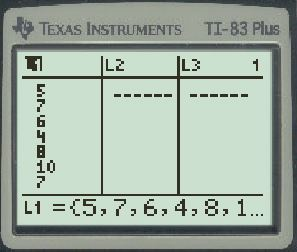
\includegraphics[scale=0.8]{Calc7} & 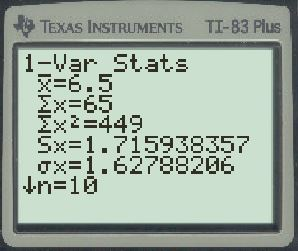
\includegraphics[scale=0.8]{Calc8}
\end{tabular}
\end{center}

The standard deviation is approximately 1.72.
\end{example}

\begin{try}[http://www.izzomath.com/103text/stats/example3.3/story.html]
The prices of a jar of peanut butter at five stores are shown below.
\begin{center}
\begin{tabular}{c c c c c}
\$3.29 & \$3.59 & \$3.79 & \$3.75 & \$3.99
\end{tabular}
\end{center}
Calculate the standard deviation of this data set.
\end{try}

\begin{exercises}

\ptwo{Which is the greatest of the following data set: the range or the standard deviation?
\[11, 11, 12, 12, 12, 12, 13, 15, 17, 22, 22, 22\]}
\ptwo{Which is the greatest of the following data set: the range or the standard deviation?
\[80, 83, 83, 87, 87, 87, 91, 97, 98\]}

\ptwo{One hundred teachers attended a seminar on mathematical problem solving. The attitudes of a representative sample of 12 of the teachers were measured before and after the seminar. A positive number for change in attitude indicates that a teacher's attitude toward math became more positive. The 12 change scores are as follows:
\[3, 8, -1, 2, 0, 5, -3, 1, -1, 6, 5, -2\]
\begin{enumerate}[(a)]
\item What is the range of the scores?
\item What is the standard deviation of the scores?
\end{enumerate}
}
\ptwo{The following are the amounts of total fat (in grams) in different kinds of sweet treats available at your local donut shop:
\begin{align*}16, 17, 16, 13, 15, 17, 16, 14, 15, 17,\\ 18, 18, 16, 16, 15, 20, 22, 19, 25, 15, 15.\end{align*}
\begin{enumerate}[(a)]
\item What is the range for this data set?
\item What is the standard deviation?
\end{enumerate}
}

\ptwo{In a neighborhood donut shop, one type of donut has 530 calories, three types of donuts have 330 calories, four types of donuts have 320 calories, seven types of donuts have 410 calories, and five types of donuts have 380 calories. Find the range and standard deviation of the calories of the donuts.} 
\ptwo{In a recent issue of \textit{IEEE Spectrum}, 84 engineering conferences were announced. Four conferences lasted 2 days, 36 lasted 3 days, 18 lasted 4 days, 19 lasted 5 days, 4 lasted 6 days, 1 lasted 7 days, 1 lasted 8 days, and 1 lasted 9 days. Find the range and standard deviation of length (in days) of an engineering conference.}

\ptwo{A researcher gathered data on hours of video games played by school-aged children and young adults. She collected the following data: \begin{align*}0, 0, 1, 1, 1, 2, 2, 3, 3, 3,\\ 4, 4, 4, 4, 5, 5, 5, 6, 6, 7,\\ 7, 7, 8, 8, 8, 8, 8, 9, 9, 9,\\ 10, 10, 11, 12, 12, 12, 12, 13.\end{align*}
\begin{enumerate}[(a)]
\item Find the range.
\item Find the standard deviation.
\item Find the five-number summary.
\end{enumerate}
}
\ptwo{The following are the sizes in square feet of the seventeen new faculty offices in the mathematics department at Frederick Community College: \begin{align*}202, 120, 120, 120, 137, 167, 122, 111, 109,\\ 108, 102, 108, 103, 103, 103, 106, 127.\end{align*}
\begin{enumerate}[(a)]
\item Find the range.
\item Find the standard deviation.
\item Find the five-number summary.
\end{enumerate}}\\

\textit{In exercises 9--10, find the five-number summary for each data set.}

\ptwo{83, 83, 87, 80, 91, 87, 97, 98}
\ptwo{1, 1, 2, 2, 2, 2, 3, 3, 3, 4, 5, 5, 5, 5}\\

\textit{In exercises 11--14, find the range and standard deviation. Then write a sentence or two explaining what those values tell you about the spread of the data.}

\ptwo{0, 0, 1, 1, 2, 2, 6, 6, 7, 7, 8, 8}
\ptwo{0, 0, 1, 1, 2, 2, 6, 7, 8}

\ptwo{0, 0, 1, 1, 8}
\ptwo{1, 1, 1, 1, 1, 1, 8}

\ptwo{Fifteen students took a statistics pre-test and post-test. The results are below. Find the range and standard deviation of the pre-test and post-test scores. Then write a sentence or two about what that tells you about the spread of the data. A score of 28 is considered a perfect score.
\begin{center}
\begin{tabular}{c | c | c}
\textbf{Student} & \textbf{Pre-test} & \textbf{Post-test}\\
\hline
& & \\
1 & 9 & 22 \\
2 & 11 & 28 \\
3 & 9 & 18 \\
4 & 4 & 24 \\
5 & 10 & 25 \\
6 & 11 & 16 \\
7 & 9 & 19 \\
8 & 9 & 20 \\
9 & 7 & 18 \\
10 & 8 & 14 \\
11 & 5 & 16 \\
12 & 15 & 26 \\
13 & 12 & 21 \\
14 & 0 & 14 \\
15 & 9 & 13
\end{tabular}
\end{center}
}
\ptwo{Below are the ages and salaries (in thousands of dollars) for CEOs of small companies. Find the range and standard deviation of age and salary. Then write a sentence or two about what this tells you about the spread of the data. Data from: http://lib.stat.cmu.edu/DASL/Datafiles/ceodat.html.
\begin{center}
\begin{tabular}{c | c | c}
\textbf{CEO} & \textbf{Age} & \textbf{Salary}\\
\hline
& & \\
1 & 53 & 145 \\
2 & 43 & 621 \\
3 & 33 & 262 \\
4 & 45 & 208 \\
5 & 46 & 362 \\
6 & 55 & 424 \\
7 & 37 & 300 \\
8 & 41 & 339 \\
9 & 55 & 736 \\
10 & 36 & 291 \\
11 & 45 & 58 \\
12 & 55 & 498 \\
13 & 50 & 643 \\
14 & 49 & 390 \\
15 & 47 & 332 \\
16 & 69 & 750
\end{tabular}
\end{center}
}

\pone{In a fifth-grade class, the teacher was interested in the range of ages of her students. The following data are the ages of a sample of 20 fifth-graders. The ages are rounded to the nearest half-year. \[9, 9.5, 9.5, 10, 10, 10, 10, 10.5, 10.5, 10.5, 10.5, 11, 11, 11, 11, 11, 11, 11.5, 11.5, 11.5.\]
Find the range, the standard deviation, and the five-number summary.} 

\pone{An experiment compared the ability of three groups of participants to remember briefly-presented chess positions. The data are shown below. The numbers represent the number of pieces correctly remembered from three chess positions. Find the range and standard deviation for each group. Then explain what this tells you about each group's ability to correctly remember chess positions.
\begin{center}
\begin{tabular}{l c c c c c c c c c c}
Non-players: & 22.1 & 22.3 & 26.2 & 29.6 & 31.7 & 33.5 & 38.9 & 39.7 & 43.2 & 43.2\\
Beginners: & 32.5 & 37.1 & 39.1 & 40.5 & 45.5& 51.3 & 52.6 & 55.7 & 55.9 & 57.7\\
Tournament players: & 40.1 & 45.6 & 51.2 & 56.4 & 58.1 & 71.1 & 74.9 & 75.9 & 80.3 & 85.3
\end{tabular}
\end{center}}
\end{exercises}

